\chapter{Introduction\label{cha:chapter1}}

% i sent you my comments by email. in general, i would recommend to restructure your introduction (and thesis) as follows:
% 1. your goal is to approximate a wide class of hysteretic processes by neural networks.
% 2. hysteretic processes have memory, introduce different hysteresis operators, say that Preisach is quite general, and it can be approximated by a linear combination of generalized (nonlinear) plays.
% 3. RNNs can approximate processes with memory, but standard architectures such as LSTM are not good enough.
% 4. that's why you develop a new architecture, namely HNN - this is your first result! it is a realization of a linear combination of nonlinear plays and hence approximates any Preisach operator (cf. item 2)
% 5. you compare hnn with lstm for learning hysteretic input-output relations and show that hnn is better. this is your second result!
% 6. you generalize a hysteretic market model from Dima and Kreiji by including N-agents. this is your third result!
% 7. you learn this model using hnn and lstm and show that hnn is better. this is your fourth result!

\textit{Hysteresis} (see \myfigref{fig:chapter1:hysteresis-loop,fig:chapter1:non-ideal-relay,fig:chapter1:stop,fig:chapter1:play}) is defined as a \textit{rate independent} process with \textit{memory effect} \citep[p. 13-14]{visintin2013differential}. It's ubiquitous in various fields, including microelectronics \citep{bondurant1989ferroelectrics,jiles1983ferromagnetic}, materials \citep{Kaltenbacher2014ATC,krejvci2007elastic,al2009generalized,ge1995modeling}, mechanics \citep{truesdell2004non,dima2014,kunze2000introduction}, economics \citep{belke2013exchange,gocke2002various,belke2014hysteresis,blanchard1986hysteresis}, etc. The nonlinear operators like \textit{non-ideal relay operator} (see \myfigref{fig:chapter1:non-ideal-relay}), \textit{stop operator} \citep{krejci1996hysteresis} (see \myfigref{fig:chapter1:stop}), \textit{play operator} \citep{krejci1996hysteresis} (see \myfigref{fig:chapter1:play}) and their generalizations are used as essential blocks to model dynamical systems with hysteresis. Preisach-type model, constructed as a superposition of non-ideal relays, is quite general in applications and it's equivalent to a linear combination of \textit{generalized plays} \citep[p. 110-111, Theorem 2.7]{visintin2013differential}.

\begin{figure}[htb!]
    \centering
    \subfloat[hysteresis loops]{
        \scalebox{1.42} {
        \documentclass{article}
\usepackage{tikz}
\begin{document}
  \begin{tikzpicture}
    \draw[] (-3,-3) .. controls (2.5,-3) and (-0.5,3) .. (3,3)
             .. controls (-2.5,3) and (0.5,-3) ..(-3,-3);
    \draw[-latex] (-4,0) -- (4,0)node[below]{$u$};
    \draw[-latex] (0,-4) -- (0,4)node[left]{$x$};
    % \draw[dashed] (-4,-3) -- (4,-3);
    % \draw[dashed] (-4,3) -- (4,3);
    
    \draw[dashed] (-3,0)node[above]{$u_1$} -- (-3,-3)node[below]{$A$};
    \node[right] at (0.7, 0) {$B$};
    \draw[dashed] (3,0)node[above]{$u_2$} -- (3,3)node[above]{$C$};
    \node[left] at (-0.7, 0) {$D$};

\end{tikzpicture}
\end{document}
        }
        \label{fig:chapter1:hysteresis-loop}
    }
    \subfloat[non-ideal relay]{
        \scalebox{1.0} {
        \documentclass{standalone}
\usepackage{pgfplots}
\pgfplotsset{compat=1.11}
\begin{document}
% Place the TikZ picture in a figure environment.
%\begin{figure}[htb]
% h: here, t: top, b: bottom, p: page of float
%% https://tex.stackexchange.com/questions/39017/how-to-influence-the-position-of-float-environments-like-figure-and-table-in-lat
%% ! indicates that some restrictions should be ignored (discussed later)
%% h indicates that the float is allowed to be placed inline
%% t indicates that the float is allowed to go into a top area
%% b indicates that the float is allowed to go into a bottom area
%% p indicates the the float is allowed to go on a float page or column area

    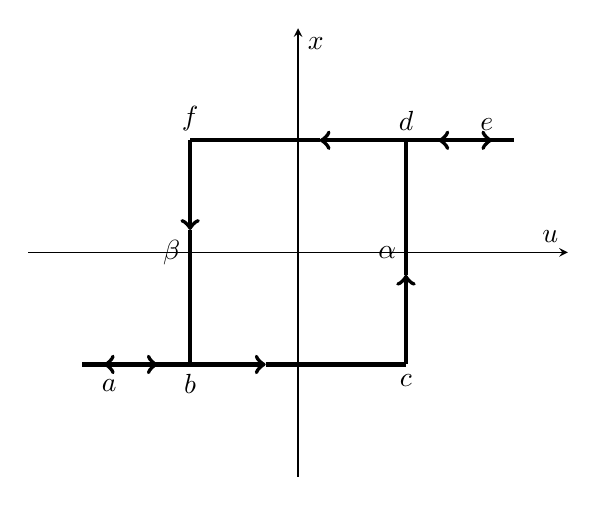
\begin{tikzpicture}
        \begin{axis} [
            xmin=-2.5, xmax=2.5, ymin=-2, ymax=2, 
            % grid=both,
            ylabel={$x$}, xlabel={$u$},
            % xtick={-2,-1.5,...,2}, ytick={-2,-1.5,...,2},
            % xticklabel style={font=\tiny, xshift=0.5ex},
            % yticklabel style={font=\tiny, yshift=0.5ex},
            axis line style={->},
            axis x line=middle,
            axis y line=middle,
            ticks=none
        ]
        \addplot+[line width=1.5pt, color=black, dashed, ->, mark=none, domain=-1.3:-1.8] {-1};
        \addplot+[line width=1.5pt,color=black, solid, ->, mark=none, domain=-2:-1.3] {-1};
        \addplot+[line width=1.5pt,color=black, solid, ->, mark=none, domain=-2:-0.3] {-1};
        \addplot+[line width=1.5pt,color=black, solid, mark=none, domain=-0.3:1] {-1};

        \addplot+[line width=1.5pt,color=black, solid, mark=none, ->,domain=1.3:1.8] {+1};

        \addplot+[line width=1.5pt,color=black, solid, mark=none, ->,domain=2:1.3] {+1};
        \addplot+[line width=1.5pt,color=black, solid, mark=none, ->, domain=1.3:0.2] {+1};
        \addplot+[line width=1.5pt,color=black, solid, mark=none, domain=0.2:-1] {+1};

        \draw[line width=1.5pt,color=black, solid, mark=none, ->] (1, -1) -- (1, -0.2);
        \draw[line width=1.5pt,color=black, solid, mark=none] (1, -0.2) -- (1, +1);

        \draw[line width=1.5pt,color=black, solid, mark=none, ->] (-1, +1) -- (-1, +0.2);
        \draw[line width=1.5pt,color=black, solid, mark=none] (-1, +0.2) -- (-1, -1);

        \node[below] at (-1.75,-1.05) {$a$};
        \node[below] at (-1,-1) {$b$};
        \node[below] at (1,-1) {$c$};
        \node[above] at (1,1) {$d$};
        \node[above] at (1.75,1) {$e$};

        \node[above] at (-1,1) {$f$};
        
        \node[left] at (-1,0) {$\beta$};
        \node[left] at (1,0) {$\alpha$};
        
        \end{axis}
    \end{tikzpicture}

\end{document}
        }
        \label{fig:chapter1:non-ideal-relay}
    }
    \hfill
    \subfloat[stop]{
       \scalebox{1.0} {
        \input{./tikz/stop-def}
        \label{fig:chapter1:stop}
        }
    }
    \subfloat[play]{
       \scalebox{1.0} {
        \documentclass{standalone}
\usepackage{pgfplots}
\pgfplotsset{compat=1.11}
\begin{document}
% Place the TikZ picture in a figure environment.
%\begin{figure}[htb]
% h: here, t: top, b: bottom, p: page of float
%% https://tex.stackexchange.com/questions/39017/how-to-influence-the-position-of-float-environments-like-figure-and-table-in-lat
%% ! indicates that some restrictions should be ignored (discussed later)
%% h indicates that the float is allowed to be placed inline
%% t indicates that the float is allowed to go into a top area
%% b indicates that the float is allowed to go into a bottom area
%% p indicates the the float is allowed to go on a float page or column area

    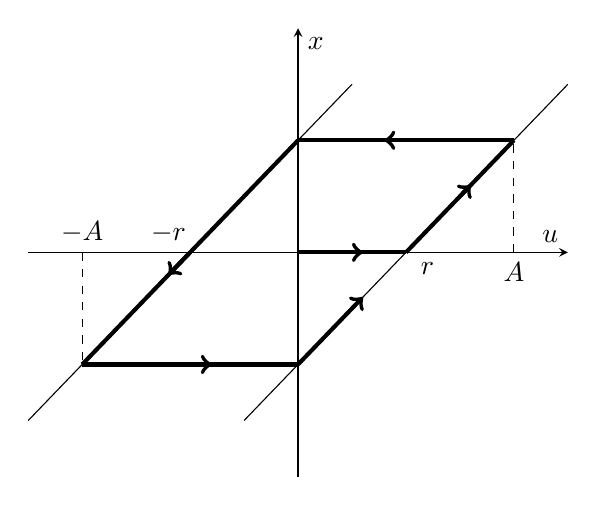
\begin{tikzpicture}
        \begin{axis} [
            xmin=-2.5, xmax=2.5, ymin=-2, ymax=2, 
            % grid=both,
            ylabel={$x$}, xlabel={$u$},
            % xtick={-2,-1.5,...,2}, ytick={-2,-1.5,...,2},
            % xticklabel style={font=\tiny, xshift=0.5ex},
            % yticklabel style={font=\tiny, yshift=0.5ex},
            axis line style={->},
            axis x line=middle,
            axis y line=middle,
            ticks=none
        ]
        \addplot+[solid, mark=none, color=black, domain=-2.5:0.5] {x+1};
        \addplot[line width=1.5pt, -> ,mark=none, color=black, domain=0:0.6] {0};
        \addplot[line width=1.5pt, - ,mark=none, color=black, domain=0.5:1] {0};

        \addplot[line width=1.5pt, -> ,mark=none, color=black, domain=1:1.6] {x-1};
        \addplot[line width=1.5pt, - ,mark=none, color=black, domain=1.5:2] {x-1};
        
        \addplot[line width=1.5pt, -> ,mark=none, color=black, domain=2:0.8] {1};
        \addplot[line width=1.5pt, - ,mark=none, color=black, domain=1:0] {1};
        
        \addplot[line width=1.5pt, -> ,mark=none, color=black, domain=0:-1.2] {x+1};
        \addplot[line width=1.5pt, - ,mark=none, color=black, domain=-1:-2] {x+1};
        
        \addplot[line width=1.5pt, -> ,mark=none, color=black, domain=-2:-0.8] {-1};
        \addplot[line width=1.5pt, - ,mark=none, color=black, domain=-1:0] {-1};
        
        \addplot[line width=1.5pt, -> ,mark=none, color=black, domain=0:0.6] {x-1};

        \node[below] at (1.2,0){$r$};
        \node[above] at (-1.2, 0){$-r$};
        \node[below] at (2,0) {$A$};
        \node[above] at (-2,0) {$-A$};
        \draw[dashed] (-2,0) -- (-2,-1);
        \draw[dashed] (2,0) -- (2,1);
        \addplot+[solid,mark=none, color=black, domain=-0.5:2.5] {x-1};
        
        \end{axis}
    \end{tikzpicture}

\end{document}
        \label{fig:chapter1:play}
        }
    }
    \caption{Interpretation of simplest \textit{hysteresis loop}, \textit{non-ideal relay}, \textit{stop} and \textit{play}. (\myfigref{fig:chapter1:hysteresis-loop}) If $u$ monotonically increases from $u_1$ to $u_2$, then the coordinate $(u, x)$ moves along the path $A \rightarrow B \rightarrow C$; conversely, if $u$ monotonically decreases from $u_2$ to $u_1$, then $(u, x)$ moves along the path $C \rightarrow D \rightarrow A$ \citep[p. 12-13]{visintin2013differential}. 
    (\myfigref{fig:chapter1:non-ideal-relay}) Hyper-parameters $\alpha$ and $\beta$ correspond to \textit{on} and \textit{off} switching values of input, respectively. As the input $u$ monotonically increased, the ascending branch $a \rightarrow b \rightarrow c \rightarrow d \rightarrow e$ is followed. When the input is monotonically decreased, the descending branch $e \rightarrow d \rightarrow f \rightarrow b \rightarrow a$ is traced  \citep[p. 2]{mayergoyz1986mathematical}. (\myfigref{fig:chapter1:stop}, \myfigref{fig:chapter1:play}) Input-output diagram for \textit{stop} and \textit{play} in the case $\dim X = 1, Z = [-r, r], u(t)=A \sin (\omega t) \, for \, A > r > 0$ \, \citep[p. 9]{krejci1996hysteresis}}
\end{figure}

In this thesis, we want to approximate a wide class of hysteretic processes, Preisach-type model, by recurrent neural network. Intuitively, recurrent neural network (RNN) is a optional approach to approximate systems with \textit{memory} since it allows previous output to be used as input while having hidden states. \citet{wang2018prandtl} applied internal time-delay RNN to describe the hysteresis and showed promising performance that their networks described both the major and minor hysteresis loops well. However, they assumed hysteretic operator is obtained in advanced so that they didn't learn this \textit{nonsmooth} operator by neural networks in their model. We also checked long short-term memory (LSTM) networks \citep{hochreiter1997long}, the state-of-the-art architecture of RNN, and found that it didn't perform well enough to reveal the relations between output and original input in hysteretic systems. % \citet{wei2000constructing} proposed a propulsive neural unit (PNU) to assist hysteresis simulation. 
In order to achieve better performance, \textbf{we develop a new neural network architecture, namely hysteretic neural network (\text{HNN}) (see \myfigref{fig:chapter1:nn-arch})}. It is a realization of a linear combination of generalized plays and hence it's able to approximate any \textit{Preisach operator} \citep{visintin2013differential}. 

% Our main contributions are 
\begin{figure}[htb!]
    \centering
    \subfloat[generalized play operator]{
        \scalebox{0.75} {
        \input{./tikz/nn-play}
        }
        % \label{fig:chapter1:nn-play}
    }
    \subfloat[linear combination of multiple generalized play operator to approximate Preisach operator]{
        \raisebox{5ex} {
        \scalebox{0.75} {
        \documentclass{standalone}
\usepackage{tikz}
\usepackage{scalerel}

% \usetikzlibrary{positioning,chains,arrows}
\begin{document}
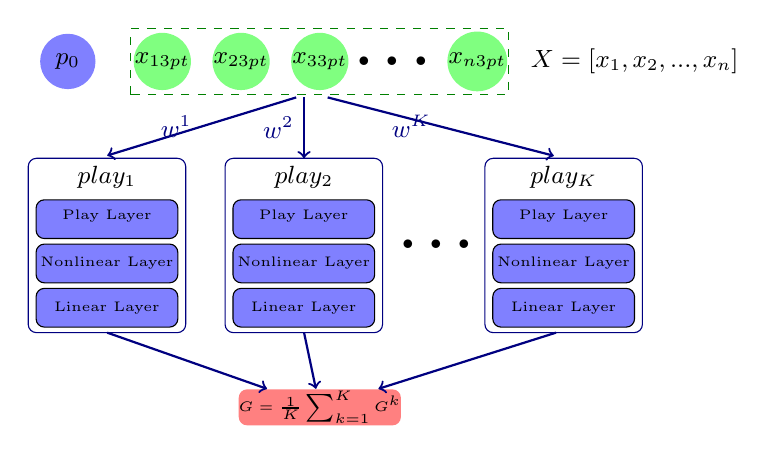
\begin{tikzpicture}[font=\small]
                       
    \tikzstyle{neuron}=[circle,fill=black!25,minimum size=20pt,inner sep=0pt]
    \tikzstyle{input neuron}=[neuron, fill=green!50];
    \tikzstyle{hidden neuron}=[neuron, fill=blue!50];
    \tikzstyle{activation neuron}=[neuron, fill=blue!50, rectangle, rounded corners=3pt, minimum size=13pt];
    \tikzstyle{play output neuron}=[neuron, fill=red!50, rectangle, rounded corners=3pt, minimum size=13pt];
    %% draw neurons
    % \draw (0.2, 0.7) node [] {Multiple Play};
    \node[hidden neuron] at (-0.2,0) {$p_0$};

    \foreach \x in {1,2,3} {
        \node[input neuron] (x_\x) at (\x, 0) {$x_{\scaleto{\x}{3pt}}$};
    }
    \node[input neuron] (x_n) at (5,0) {$x_{\scaleto{n}{3pt}}$};
    \path (x_3) -- (x_n) node[midway,scale=2,font=\bfseries] {\dots};
    \draw[dashed,thin,green!50!black] (0.6,-12pt) rectangle (5.4, 12pt);
    \node[] (input) at (2.8,-10pt) {}; % make anchor here
    \node[] at (7, 0) {$X=[x_1,x_2,...,x_n]$};
    
    \begin{scope}[xshift=-20]
    \foreach \x / \idx in {0/1,2.5/2} {
        \draw[thick,solid,rounded corners=3pt,thin,blue!50!black] (\x,-35pt) rectangle (\x+2, -98pt);
        % \node[] (play_\idx) at (\x+1, -35pt);
        \node[] at (\x+1, -42pt) {$play_\idx$};
        
        \draw[solid,rounded corners=3pt,thin,fill=blue!50!white] (\x+0.1,-50pt) rectangle (\x+1.9, -64pt);
        \node[]  at (\x+1,-56pt) {\tiny Play Layer};
        \draw[solid,rounded corners=3pt,thin,fill=blue!50!white] (\x+0.1,-66pt) rectangle (\x+1.9, -80pt);
        \node[]  at (\x+1,-73pt) {\tiny Nonlinear Layer};
        \draw[solid,rounded corners=3pt,thin,fill=blue!50!white] (\x+0.1,-82pt) rectangle (\x+1.9, -96pt);
        \node[]  at (\x+1,-89pt) {\tiny Linear Layer};
    }
    
    \draw[thick,solid,rounded corners=3pt,thin,blue!50!black] (5.8,-35pt) rectangle (7.8, -98pt);
    \node[] (play_k) at (6.8, -35pt) {};
    \node[] at (6.8, -42pt) {$play_K$};
    \draw[solid,rounded corners=3pt,thin,fill=blue!50!white] (5.9,-50pt) rectangle (7.7, -64pt);
    \node[]  at (6.8,-56pt) {\tiny Play Layer};
    \draw[solid,rounded corners=3pt,thin,fill=blue!50!white] (5.9,-66pt) rectangle (7.7, -80pt);
    \node[]  at (6.8,-73pt) {\tiny Nonlinear Layer};
    \draw[solid,rounded corners=3pt,thin,fill=blue!50!white] (5.9,-82pt) rectangle (7.7, -96pt);
    \node[]  at (6.8,-89pt) {\tiny Linear Layer};
    \end{scope}

    \path (4.3,-66pt) -- (4.8, -66pt) node[midway,scale=2,font=\bfseries] {\dots};

    \draw [->,color=blue!50!black,thick] (2.7,-13pt) to node [left,color=blue!50!black] {$w^1$} (0.3,-34pt);
    \draw [->,color=blue!50!black,thick] (2.8,-13pt) to node [left,color=blue!50!black] {$w^2$} (2.8,-35pt);
    \draw [->,color=blue!50!black,thick] (3.1,-13pt) to node [left,color=blue!50!black] {$w^K$} (play_k);
    
    \node[play output neuron] (output) at (3, -125pt) {\tiny $G=\frac{1}{K}\sum_{k=1}^{K}G^{k}$};
    
    \draw [->,color=blue!50!black,thick] (0.3,-98pt) to node [left,color=blue!50!black] {} (output);
    \draw [->,color=blue!50!black,thick] (2.8,-98pt) to node [left,color=blue!50!black] {} (output);
    \draw [->,color=blue!50!black,thick] (6.,-98pt) to node [left,color=blue!50!black] {} (output);
\end{tikzpicture}
\end{document}


        }
        }
        % \label{fig:chapter1:nn-arch}
    }
    \caption{}
    \label{fig:chapter1:nn-arch}
\end{figure}

% second results
Given an observation $(x_n, y_n) \, (n=1,\ldots, N)$ underlying hysteretic input-output relations, both LSTM and HNN minimize mean square error (MSE) between predicted target $\hat{y}_n$ and observed target $y_n$. \textbf{It shows HNN outperforms LSTM by comparing root mean square error (RMSE) (see \myfigref{fig:chapter1:hnn-lstm-results}). In particular, HNN is able to reconstruct minor hysteresis loops well whereas LSTM fails.} 

\begin{figure}[htb!]
    \centering
    \subfloat[]{
        \scalebox{1.0} {
        \includegraphics[width=\textwidth]{analysis_hnn_lstm_dima_sequence}
        }
        \label{fig:chapter1:hnn-lstm-result-1}
    }
    \hfill
    \subfloat[]{
        \scalebox{1.0} {
        \includegraphics[width=\textwidth]{analysis_hnn_lstm_pavel_sequence}
        }
        \label{fig:chapter1:hnn-lstm-result-2}
    }
    \caption{The overall predictive outputs against ground-truth outputs. \mytodo{detail interpretation of input and output sequence or not ?}} \label{fig:chapter1:hnn-lstm-results}
\end{figure}

Based on the HNN we obtain, we study a particular application, momentum-based trading strategies in financial market, with hysteretic property in economic. \citet{dima2014} proposed a market model and used Prandtl-Ishlinskii operator, a particular case of the Preisach model, to model trading strategies within their market model. It provides a promising insight to make play-hysteresis economic models compatible with multi-agent modeling framework \citep{cross2007stylized,cartwright1999dappled,lamba2008market}. However, they only considered single trading strategy that agents take reaction to the change of \textit{price trend}, called \textit{agents D} (cf.  \ref{assumption:chapter3:strategy-of-agentD}) in this thesis, to simulate market movements. Another trading strategy, which is common in financial trading pattern as well, is also threshold-based where agents in markets are sensitive to the fluctuation of some \textit{fixed price value} instead of \textit{price trend}, called \textit{agents N} (cf. \ref{assumption:chapter3:strategy-of-agentN}) in this thesis. \textbf{We generalize \citet{dima2014}'s market model by introducing two different agents, agents D and agents N based on generalized play operator and non-ideal relay operator respectively.}

\textbf{Again, we learn this financial market model using HNN and LSTM, by  maximizing log-likelihood of price distribution to train both networks. It reveals HNN models this kind of market model better than LSTM.} Even HNN is possible to reconstruct the \textit{unobserved state changes underlying the market}, which is useful to interpret the \textit{avalanche of market movements}, since it inherently contains agents that use different trading strategies in micro level. 

% organization
The thesis is organized as follows. In the next chapter, a detail methodology for HNN is discussed, including how to formulate hysteretic systems by generalized play operator and learn the neural networks. In chapter 3, we presents detail discussions about our financial market model and provide a practical approach to generate synthetic data for further evaluation. In chapter 4, we formulate the methods to learn our market model. In chapter 5, we evaluate performance between LSTM and HNN in different degrees, including the complexity of data sets, network complexity and the accuracy of predicted results. The last chapter contains our conclusions and future works.